\documentclass[xcolor=x11names,compress]{beamer}

%% General document %%%%%%%%%%%%%%%%%%%%%%%%%%%%%%%%%%
\usepackage{graphicx}
\usepackage{tikz}
\usepackage{Tabbing}
\usetikzlibrary{decorations.fractals}
\usepackage{fancyvrb}
%%%%%%%%%%%%%%%%%%%%%%%%%%%%%%%%%%%%%%%%%%%%%%%%%%%%%%

%% Beamer Layout %%%%%%%%%%%%%%%%%%%%%%%%%%%%%%%%%%
\useoutertheme[subsection=false,shadow]{miniframes}
\useinnertheme{default}
\usefonttheme{serif}
\usepackage{palatino}
\usepackage{tabu}
% Links
\usepackage{hyperref}
\definecolor{links}{HTML}{003262}
\hypersetup{colorlinks,linkcolor=,urlcolor=links}

% addition of color
\usepackage{xcolor}
\definecolor{CoolBlack}{rgb}{0.0, 0.18, 0.39}
\definecolor{byellow}{rgb}{0.55037, 0.38821, 0.06142}
\definecolor{dgreen}{rgb}{0.,0.6,0.}
\definecolor{RawSienna}{cmyk}{0,0.72,1,0.45}
\definecolor{forestgreen(web)}{rgb}{0.13, 0.55, 0.13}
\definecolor{cardinal}{rgb}{0.77, 0.12, 0.23}

\setbeamerfont{title like}{shape=\scshape}
\setbeamerfont{frametitle}{shape=\scshape}

\setbeamercolor*{lower separation line head}{bg=CoolBlack}
\setbeamercolor*{normal text}{fg=black,bg=white}
\setbeamercolor*{alerted text}{fg=dgreen} % just testing; I think this looks better
\setbeamercolor*{example text}{fg=black}
\setbeamercolor*{structure}{fg=black}

\setbeamercolor*{palette tertiary}{fg=black,bg=black!10}
\setbeamercolor*{palette quaternary}{fg=black,bg=black!10}

% Margins
\usepackage{changepage}

\mode<presentation>
{
  \definecolor{berkeleyblue}{HTML}{003262}
  \definecolor{berkeleygold}{HTML}{FDB515}
  \usetheme{Boadilla}      % or try Darmstadt, Madrid, Warsaw, Boadilla...
  %\usecolortheme{dove} % or try albatross, beaver, crane, ...
  \setbeamercolor{structure}{fg=berkeleyblue,bg=berkeleygold}
  \setbeamercolor{palette primary}{bg=berkeleyblue,fg=white} % changed this
  \setbeamercolor{palette secondary}{fg=berkeleyblue,bg=berkeleygold} % changed this
  \setbeamercolor{palette tertiary}{bg=berkeleyblue,fg=white} % changed this
  \usefonttheme{structurebold}  % or try serif, structurebold, ...
  \useinnertheme{circles}
  \setbeamertemplate{navigation symbols}{}
  \setbeamertemplate{caption}[numbered]
  \usebackgroundtemplate{}
}


\usepackage{cutwin}

% adding slide numbers
\addtobeamertemplate{navigation symbols}{}{%
    \usebeamerfont{footline}%
    \usebeamercolor[fg]{footline}%
    \hspace{1em}%
    \insertframenumber/\inserttotalframenumber
}

% equation stuff
\usepackage{mathrsfs}
\usepackage[mathcal]{euscript}
\usepackage{amssymb}
\usepackage{amsthm}
\usepackage{epsfig}
\usepackage{amsmath}

% title stuff for footer
\title{The PyNE Software Library}
\author{C.\ R.\ Bates}
\date{11 November 2014}

% arrow
\usetikzlibrary{shapes.arrows}
\tikzset{
        myarrow/.style={
        draw,
        fill=orange,
        single arrow,
        minimum height=3.5ex,
        single arrow head extend=0.5ex}
}

\newcommand{\arrowdown}{
 \tikz [baseline=-1ex]{\node [myarrow,rotate=-90] {};}
}

%%%%%%%%%%%%%%%%%%%%%%%%%%%%%%%%%%%%%%%%%%%%%%%%%%%%%
\begin{document}



%%%%%%%%%%%%%%%%%%%%%%%%%%%%%%%%%%%%%%%%%%%%%%%%%%%%%%
%%%%%%%%%%%%%%%%%%%%%%%%%%%%%%%%%%%%%%%%%%%%%%%%%%%%%%
\begin{frame}
\title{PyNE Progress Report}
%\subtitle{}
\author{\textbf{Anthony~Scopatz$^{1}$} for Cameron~R.~Bates$^{2,3}$ \\
        \vspace{0.1in}
        Elliott~Biondo$^{1}$, Kathryn~Huff$^{2}$,
        Kalin Kiesling$^{1}$,
        Robert Carlsen$^{1}$,
        Andrew Davis$^{1}$,
        Matthew Gidden$^{1}$,
        Tim Haines$^{1}$,
        Joshua Howland$^{2}$,
        Blake Huff$^{2}$,
        Kevin Manalo$^{4}$,
        Arielle Opotowsky$^{1}$,
        Rachel Slaybaugh$^{2}$,
        Eric Relson$^{1}$,
        Paul Romano$^{5}$,
        Patrick Shriwise$^{1}$,
        John D. Xia$^{6}$,
        Paul Wilson$^{1}$,
        Julie Zachman$^{1}$\\
        \vspace{0.1in}
        $^{1}$ The University of Wisconsin-Madison\\
        $^{2}$ The University of California, Berkeley\\
        $^{3}$ Lawrence Livermore National Laboratory\\
        $^{4}$ Georgia Institute of Technology\\
        $^{5}$ Massachusetts Institute of Technology\\
        $^{6}$ University of Chicago}

\date{ANS Winter Meeting, November 11, 2014}
\titlepage
\end{frame}

%------------------------------------------------------
\begin{frame}{Outline}

	\begin{columns}
  	\begin{column}{0.5\textwidth}
	    \begin{itemize}
        \item PyNE \cite{pyne}: what is it?

        (Python for Nuclear Engineering)
        \item New Features
        \item Improved Usability
        \item Future plans
        \item Expanding the community
	    \end{itemize}
  	\end{column}
 	%
 	\begin{column}{0.4\textwidth}
 	   \begin{center}
 	   \begin{figure}
       
\includegraphics[height=4cm]{pyne-icon-big.png}
	   \end{figure}
 	   \end{center}
  	\end{column}
	\end{columns}

\end{frame}

%%%%%%%%%%%%%%%%%%%%%%%%%%%%%%%%%%%%%%%%%%%%%%%%%%%%%%
%%%%%%%%%%%%%%%%%%%%%%%%%%%%%%%%%%%%%%%%%%%%%%%%%%%%%%
\section{PyNE \cite{pyne}: what is it?}
\begin{frame}{What is PyNE?}

    PyNE is \textcolor{dgreen}{the} open source nuclear engineering toolkit.
    \vspace*{1em}
    \begin{itemize}
    \item PyNE is a \textcolor{dgreen}{library of composable tools} used to build
    nuclear science and engineering applications
    \item It is \textcolor{dgreen}{permissively licensed} (2-clause BSD)
    \item It supports both a \textcolor{dgreen}{C++} and a \textcolor{dgreen}{Python} API
    \item The name `PyNE' is a bit of a misnomer since most of the code
    base is in C++ but most daily usage happens in Python
    \item \textcolor{dgreen}{v0.4} is the current, stable release
    \item As an organization, PyNE was born in April 2011
    (however, core parts of PyNE have existed since 2007)
    \end{itemize}

\end{frame}

%------------------------------------------------------
\begin{frame}{What are the Goals of PyNE?}

    \begin{columns}
    \begin{column}{0.45\textwidth}
        To help nuclear engineers:
        \begin{itemize}
        \item be more \alert{productive} (don't reinvent the wheel!)
        \item have the \alert{best solvers}
        \item have a \alert{clear and useful API}
        \item write really \alert{great code}
        \item \alert{teach} the next generation
        \end{itemize}
  	\end{column}
   	%
 	\begin{column}{0.45\textwidth}
 	   \begin{center}
 	   \begin{figure}
 	   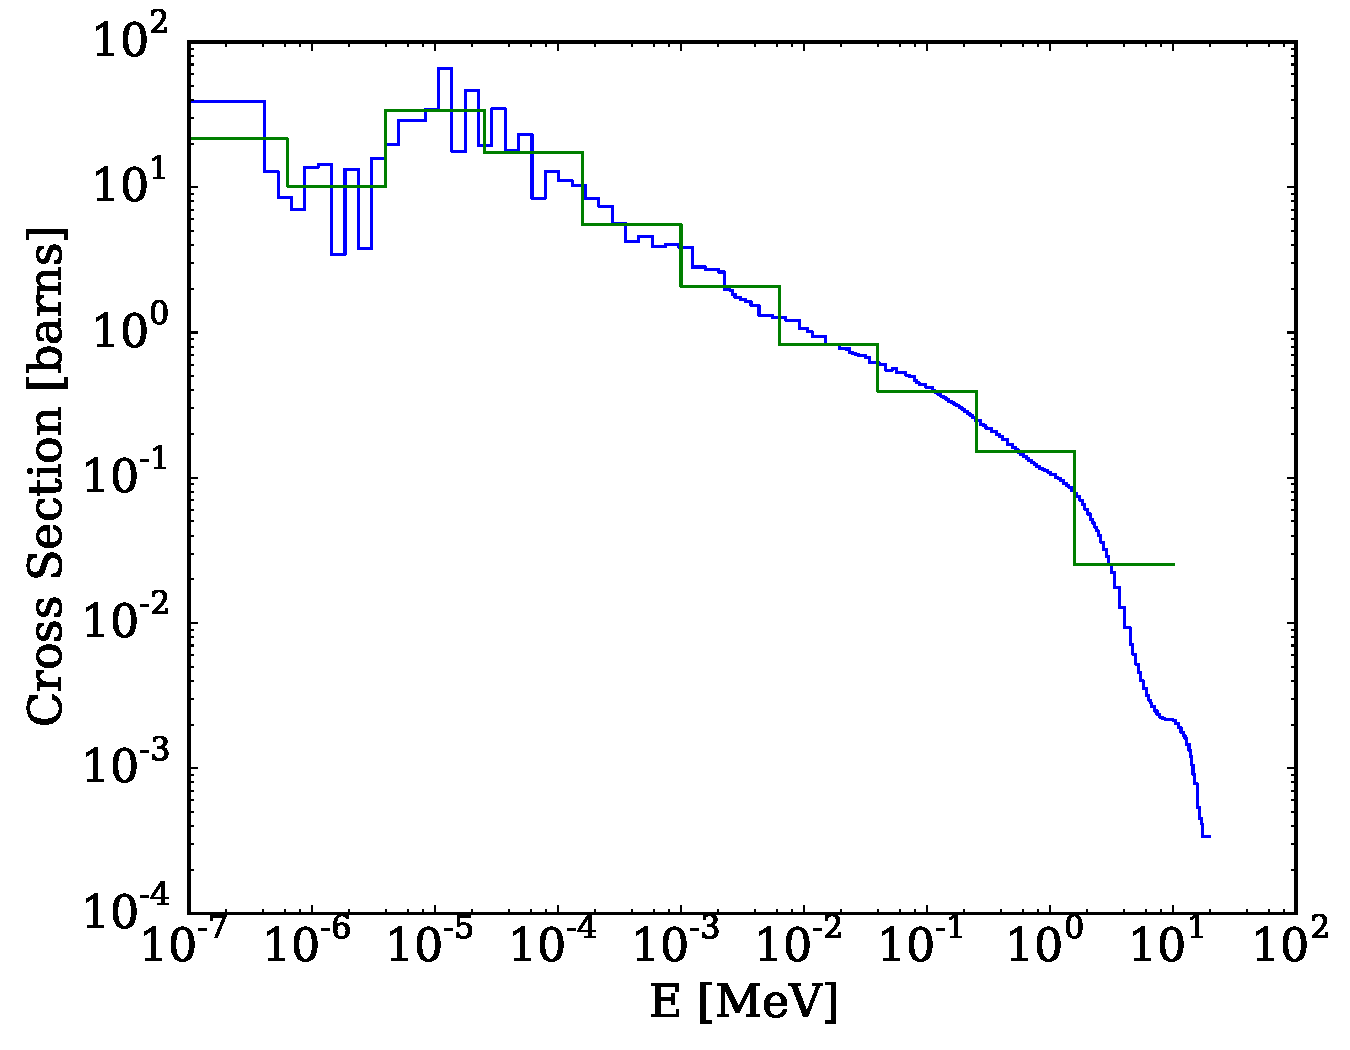
\includegraphics[height=1.75in,clip]{xs.pdf}  \\
	   \end{figure}
 	   \end{center}
  	\end{column}
	\end{columns}

\end{frame}

%%%%%%%%%%%%%%%%%%%%%%%%%%%%%%%%%%%%%%%%%%%%%%%%%%%%%%
%%%%%%%%%%%%%%%%%%%%%%%%%%%%%%%%%%%%%%%%%%%%%%%%%%%%%%
\section{Demo}
\begin{frame}{What Can PyNE Do?}

    The idea is to be able to easily combine components and avoid redeveloping
    utilities someone else has developed. \textbf{new/improved}

    \begin{itemize}
    \item Nuclear data and cross-section reading/processing
    \begin{itemize}
        \item \textbf{ENSDF}, ENDF, \textbf{ACE}
    \end{itemize}
    \item Material management
    \begin{itemize}
        \item \textbf{FLUKA}, MCNP
    \end{itemize}
    \item Canonical nuclide, particle and reaction naming conventions
    \item \textbf{Mesh operations}
    \begin{itemize}
        \item \textbf{DAGMC, ALARA, CADIS}
    \end{itemize}
    \item MCNP and Serpent input/output parsing
    \item Fuel cycle functionality (transmutation, enrichment)
    \item \textbf{AHOT}
    \item \textbf{Rigorous Two-Step Activation}
    \item \textbf{MORE!}
    \end{itemize}

\end{frame}

%------------------------------------------------------
%%%%%%%%%%%%%%%%%%%%%%%%%%%%%%%%%%%%%%%%%%%%%%%%%%%%%%
%%%%%%%%%%%%%%%%%%%%%%%%%%%%%%%%%%%%%%%%%%%%%%%%%%%%%%
\begin{frame}{Improvements in ENSDF}
    %old vs. new plot of nuclide half-lives
    \begin{itemize}
        \item Completely re-written parser
        \item Reads all level and decay information into HDF5
    \end{itemize}

    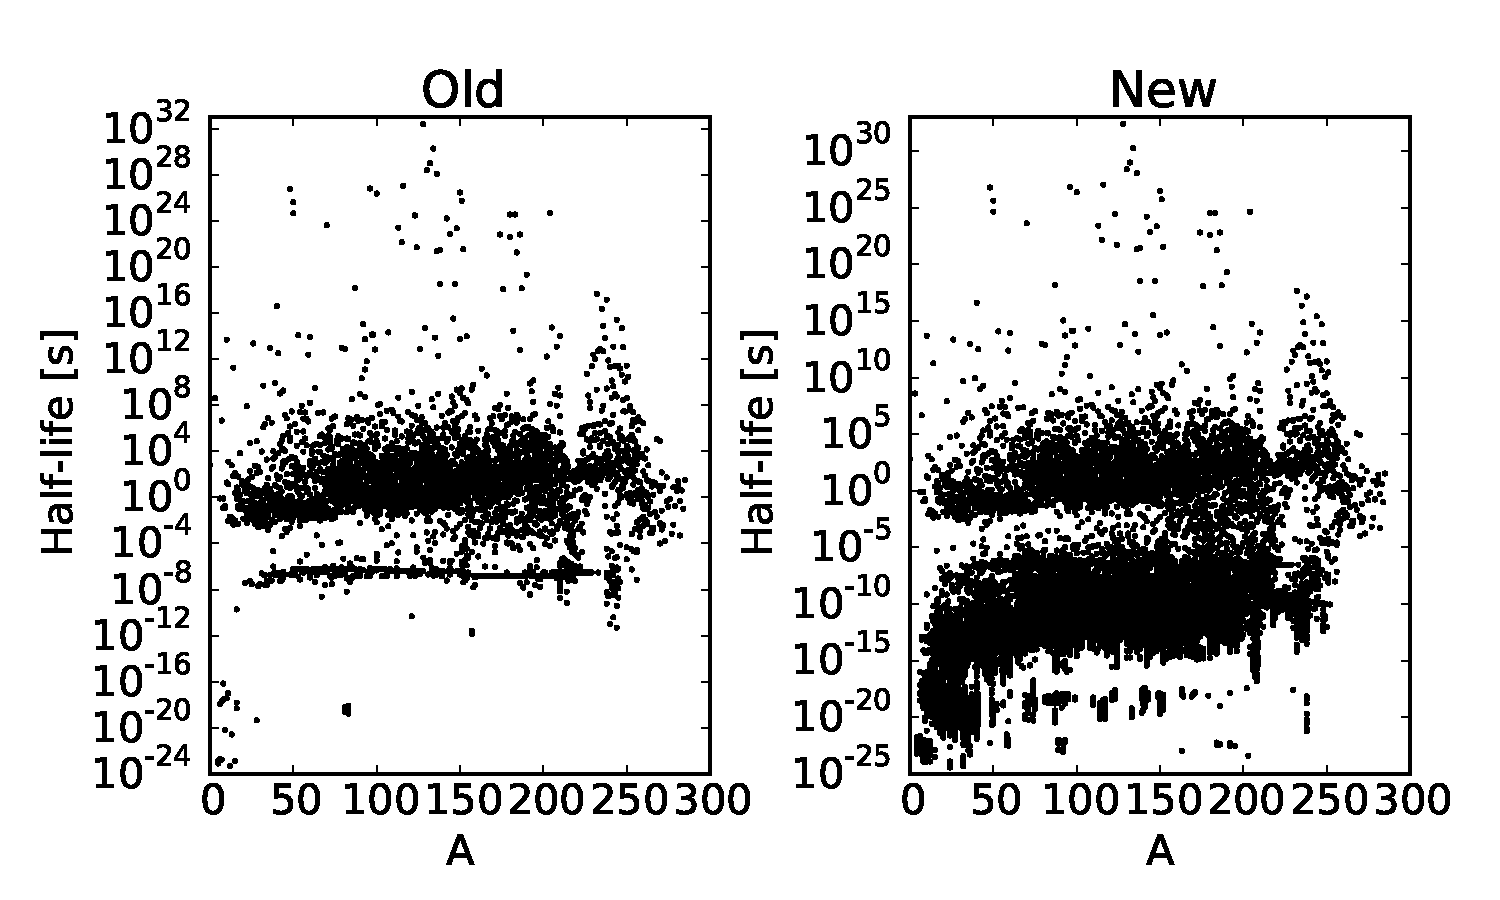
\includegraphics[height=2.5in,clip]{ensdf.pdf}

\end{frame}

\begin{frame}{Addition of Fission Yield data}
    \begin{columns}
        \begin{column}{0.45\textwidth}
            \begin{center}
                WIMSD LWR (ENDF/B-VII.0)
                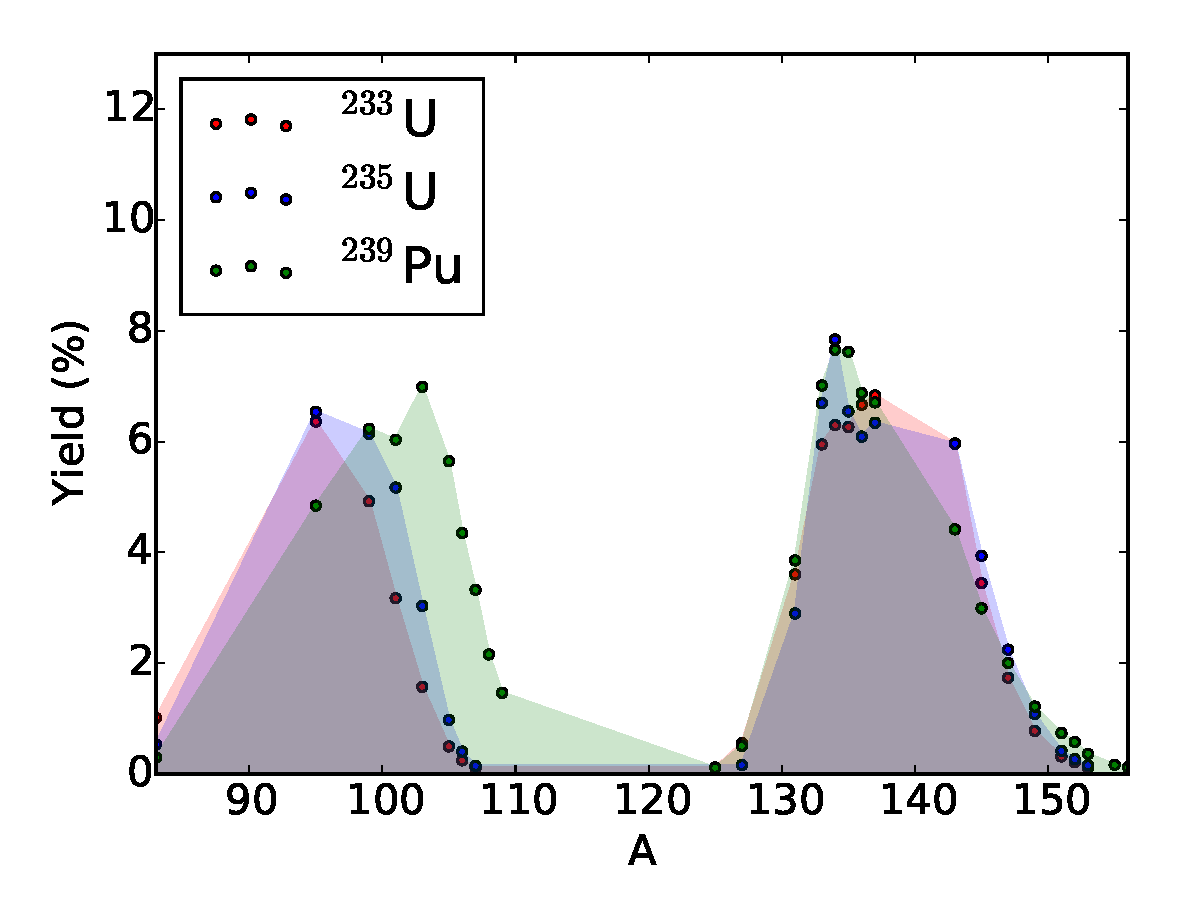
\includegraphics[height=1.75in,clip]{yieldwimsd.pdf}
            \end{center}
  	    \end{column}
 	    \begin{column}{0.45\textwidth}
            \begin{center}
            NDS Thermal (JEFF-3.1)
            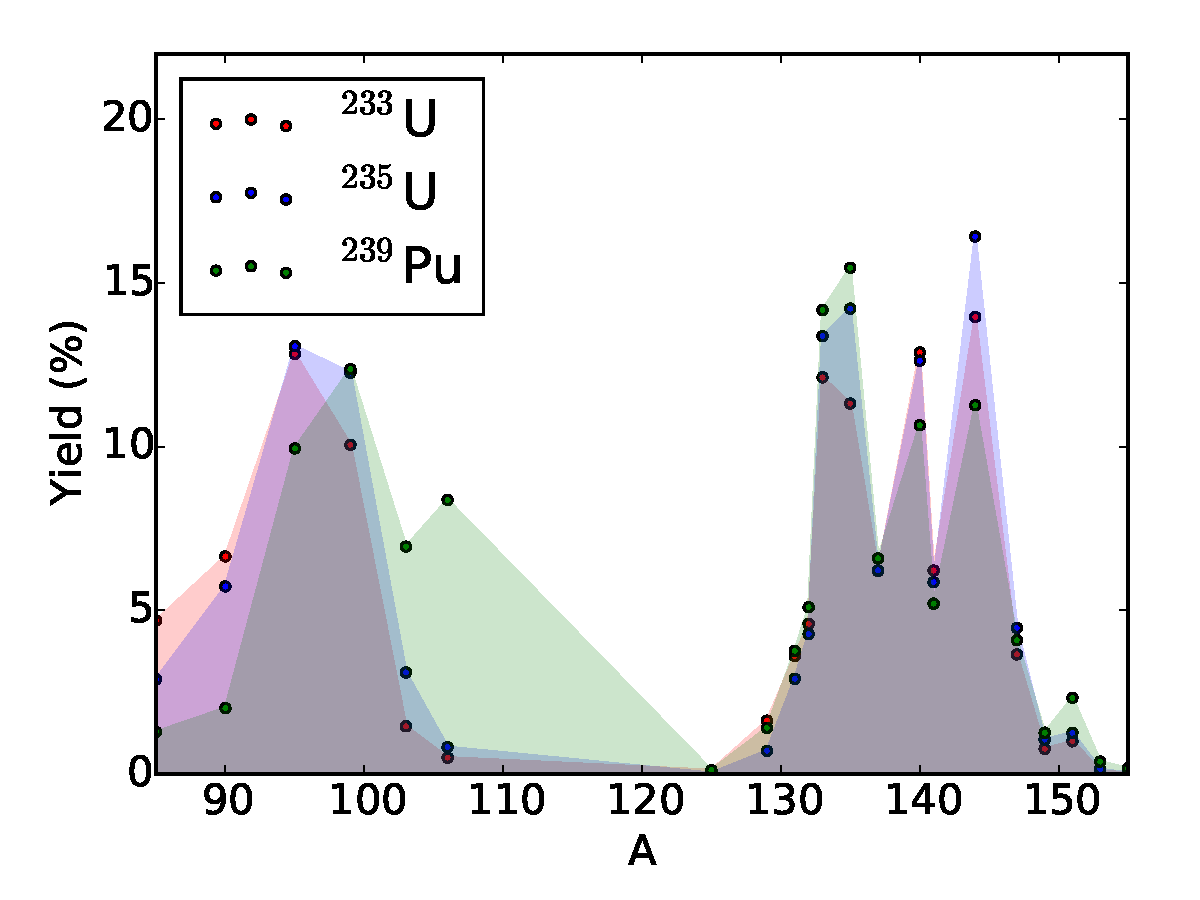
\includegraphics[height=1.75in,clip]{yieldnds.pdf}
            \end{center}
        \end{column}
    \end{columns}
\end{frame}

%%%%%%%%%%%%%%%%%%%%%%%%%%%%%%%%%%%%%%%%%%%%%%%%%%%%%%
%%%%%%%%%%%%%%%%%%%%%%%%%%%%%%%%%%%%%%%%%%%%%%%%%%%%%%
\begin{frame}{Meshes in PyNE}
    \begin{columns}
        \begin{column}{0.45\textwidth}
            \begin{itemize}
                \item Facilitates manipulating and plotting of meshes (with yt's help)
                \item Reads MCNP mesh tallies
                \item Writes MCNP mesh inputs
            \end{itemize}
  	    \end{column}
   	%
 	    \begin{column}{0.45\textwidth}
            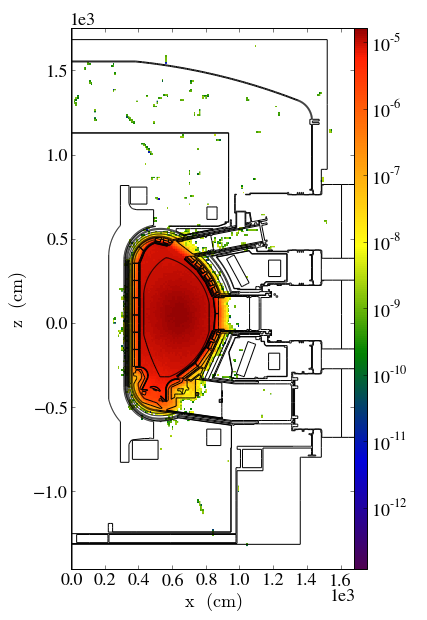
\includegraphics[height=2.5in,clip]{flux_slice.png}
        \end{column}
    \end{columns}


    % ITER plot
    % Talk about how awesome yt is (and we are by association)
\end{frame}

\begin{frame}{Discretizing Geometry}
    \begin{itemize}
        \item Discretize geometry on tetrahedral or cartesian mesh for transport
        \item Relies on CUBIT for mesh generation
        \item Redistributes volume averaged properties
    \end{itemize}
    \begin{columns}
        \begin{column}{0.45\textwidth}
            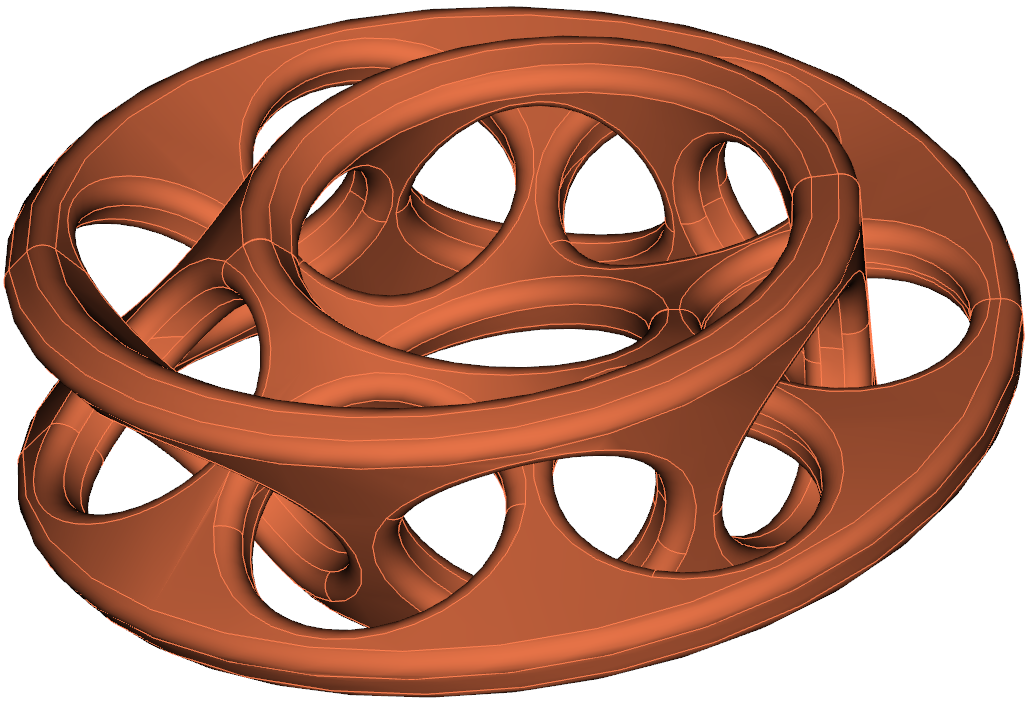
\includegraphics[height=1.1in,clip]{mobius_cad.png}
  	    \end{column}
   	%
 	    \begin{column}{0.45\textwidth}
            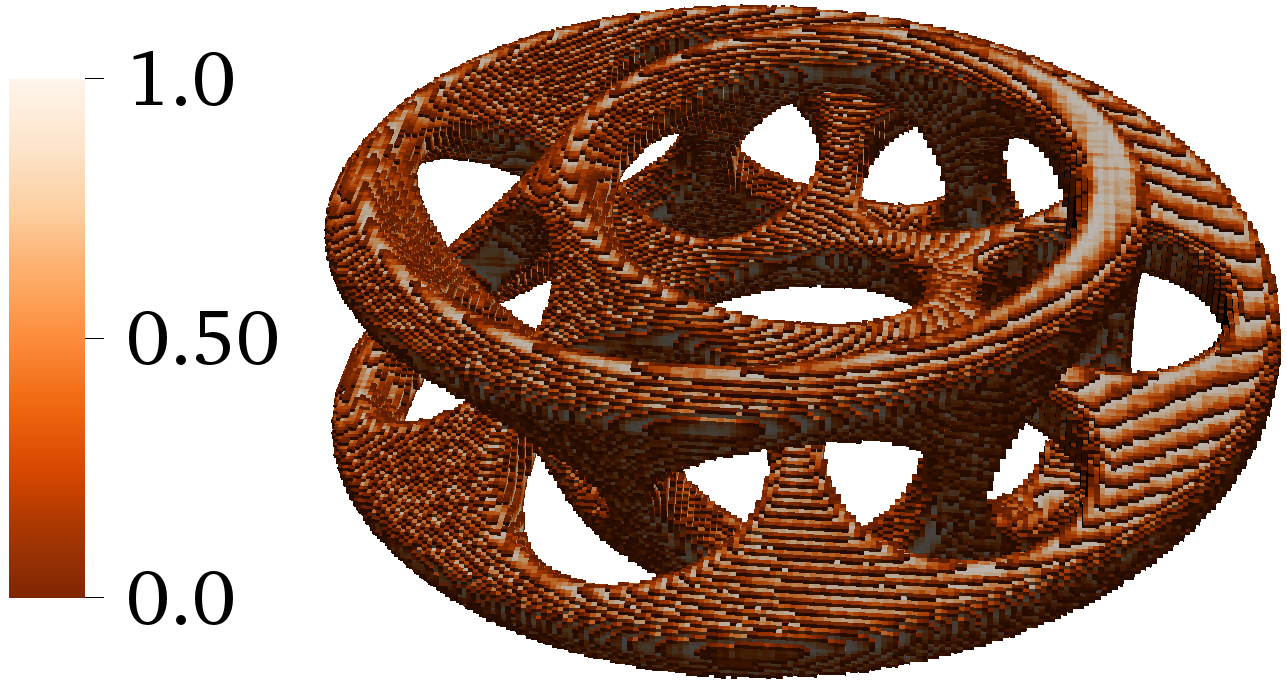
\includegraphics[height=1.1in,clip]{mobius_mesh.png}
        \end{column}
    \end{columns}
    % Elliott's sweet discretized geometry
    % Explain that it's tetrahedral or cartesian --> Sn transport friendly!
\end{frame}

%%%%%%%%%%%%%%%%%%%%%%%%%%%%%%%%%%%%%%%%%%%%%%%%%%%%%%
\begin{frame}
\frametitle{Mesh-based source sampling}

Randomly sample Monte Carlo birth parameters (position, energy, statistical weight) from a mesh-based source.\\
\vspace{0.3cm}
The PyNE \texttt{Sampler} class:
\begin{itemize}
\item{Cartesian and tetrahedral mesh}
\item{Utilizes alias sampling method \cite{smith_analysis_2005}}
\item{Sampling modes:}
  \begin{itemize}
  \item{analog -- no source biasing}
  \item{uniform -- all phases space sampled equally, statistical weight adjusted accordingly}
  \item{user-specified -- any bias scheme specified by the user}
    \begin{itemize}
    \item{Consistent Adjoint-Driven Importance Sampling (CADIS) in PyNE \texttt{variance\_reduction} module}
    \end{itemize}
  \end{itemize}
\end{itemize}
\end{frame}

%%%%%%%%%%%%%%%%%%%%%%%%%%%%%%%%%%%%%%%%%%%%%%%%%%%%%%
\begin{frame}
\frametitle{Source sampling modes}

\begin{columns}[T]
\begin{column}{0.3\textwidth}
\begin{block}{\tiny Source density distribution}
\vspace{0.2cm}
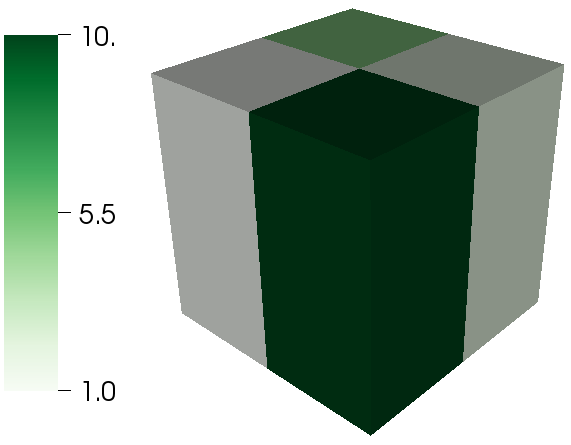
\includegraphics[height=2.5cm]{sampler_src.png}
\end{block}
\end{column}
\begin{column}{0.3\textwidth}
\begin{block}{\tiny Analog sampling}
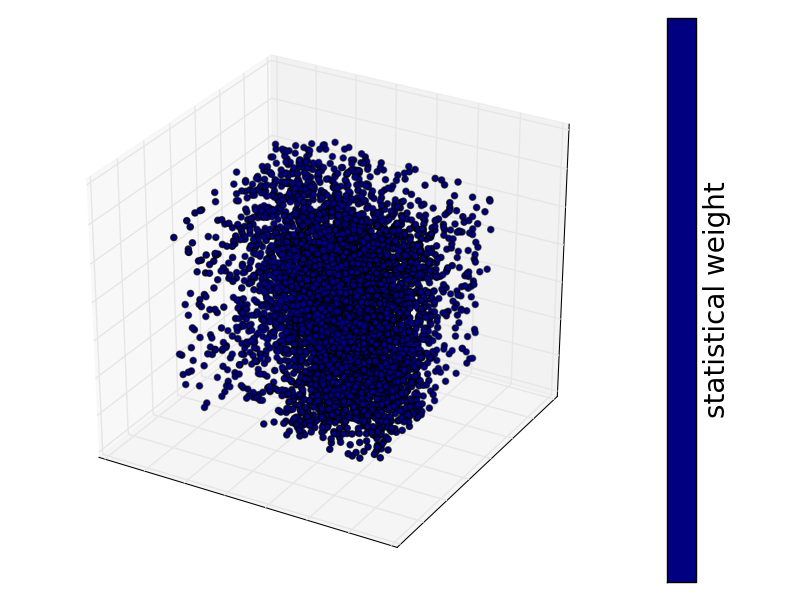
\includegraphics[height=2.7cm]{sample_cart.png}
\end{block}
\end{column}
\begin{column}{0.3\textwidth}
\begin{block}{\tiny Uniform sampling}
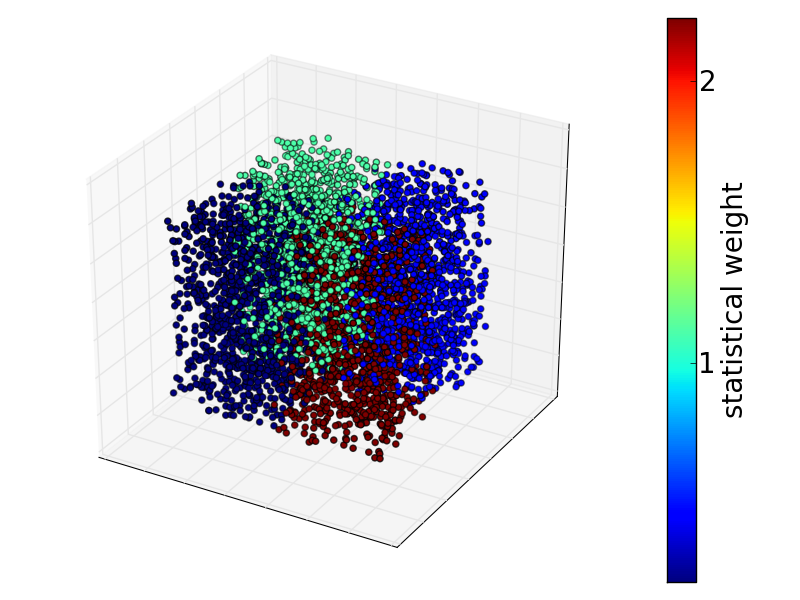
\includegraphics[height=2.7cm]{sample_uniform.png}
\end{block}
\end{column}
\end{columns}

\begin{columns}[T]
\begin{column}{0.3\textwidth}
\vspace{0.6cm}
{\small In addition to a source density distribution, a biased source density distribution can also be specified.}
\end{column}
\begin{column}{0.3\textwidth}
\begin{block}{\tiny Biased source density distribution}
\vspace{0.2cm}
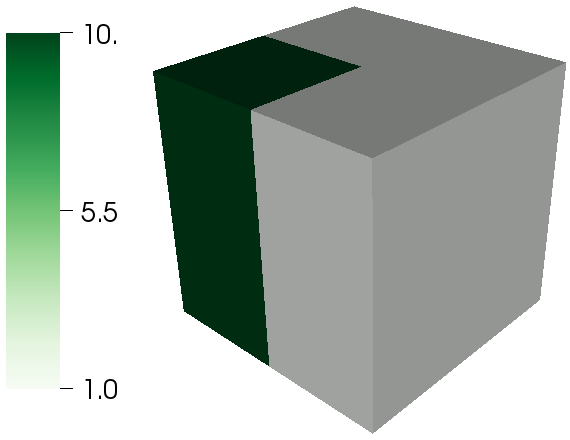
\includegraphics[height=2.5cm]{sampler_bias.png}
\end{block}
\end{column}
\begin{column}{0.3\textwidth}
\begin{block}{\tiny used-specified sampling}
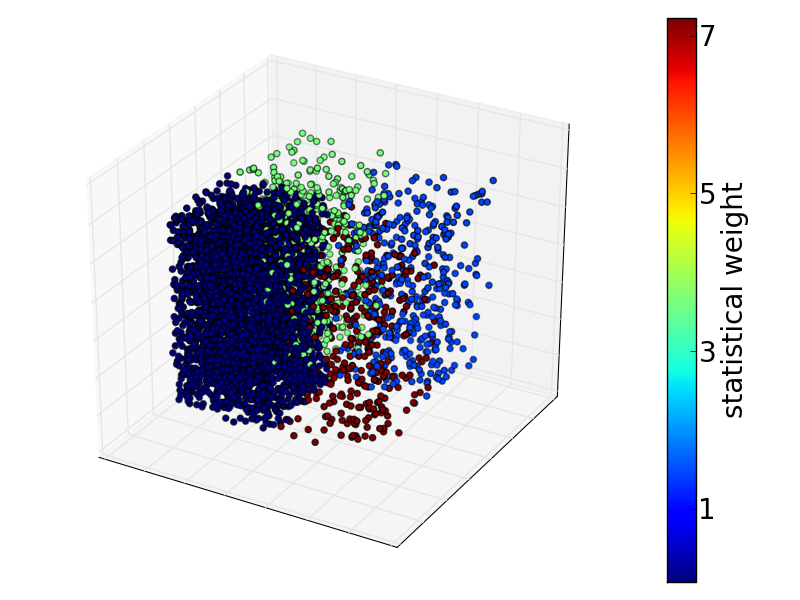
\includegraphics[height=2.7cm]{sample_user.png}
\end{block}
\end{column}
\end{columns}

\end{frame}

%%%%%%%%%%%%%%%%%%%%%%%%%%%%%%%%%%%%%%%%%%%%%%%%%%%%%%
\begin{frame}
\frametitle{Using the \texttt{Sampler} class}
\Large
\begin{itemize}
\item{Written in C++}
\item{Intended to be integrated into physics codes}
  \begin{itemize}
    \large
    \item{C/C++, Fortran, Python interfaces}
  \end{itemize}
\item{Use with MCNP5 via supplied source.F90 file}
\end{itemize}
\end{frame}

%%%%%%%%%%%%%%%%%%%%%%%%%%%%%%%%%%%%%%%%%%%%%%%%%%%%%%
\begin{frame}
\frametitle{Complex source definitions}

Define a source instead of an \texttt{sdef}, the sky is the limit!

\begin{columns}[T]
    \begin{column}{.4\textwidth}
     \begin{block}{CAD geometry}
    \centering{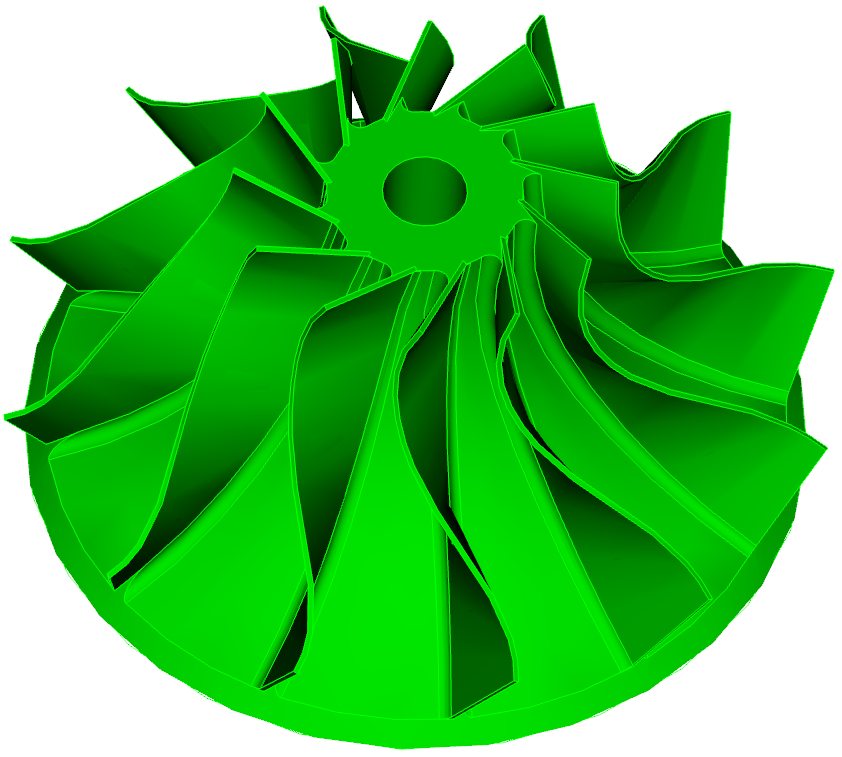
\includegraphics[width=4.5cm]{turbine_cad.png}}
     \vspace{0.1cm}
     \end{block}
    \end{column}
    \begin{column}{.45\textwidth}
    \begin{block}{source density (p/cm$^3$/s)}
    \centering{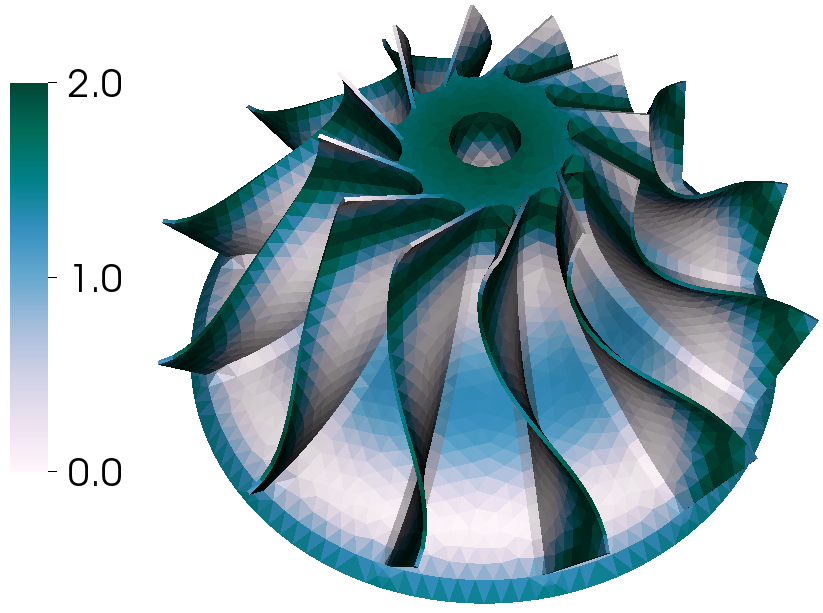
\includegraphics[width=5.5cm]{turbine_src.png}}
    \end{block}
    \end{column}
\end{columns}

\end{frame}

%%%%%%%%%%%%%%%%%%%%%%%%%%%%%%%%%%%%%%%%%%%%%%%%%%%%%%
\begin{frame}
\frametitle{Complex source definitions}
Photon flux distribution from MCNP5:
\begin{columns}[c]

\centering
\begin{column}{0.1\textwidth}
\rotatebox{90}{(\large p/cm$^2$/history)}
\end{column}

\begin{column}{0.8\textwidth}
\hspace{-0.85cm}
\centerline{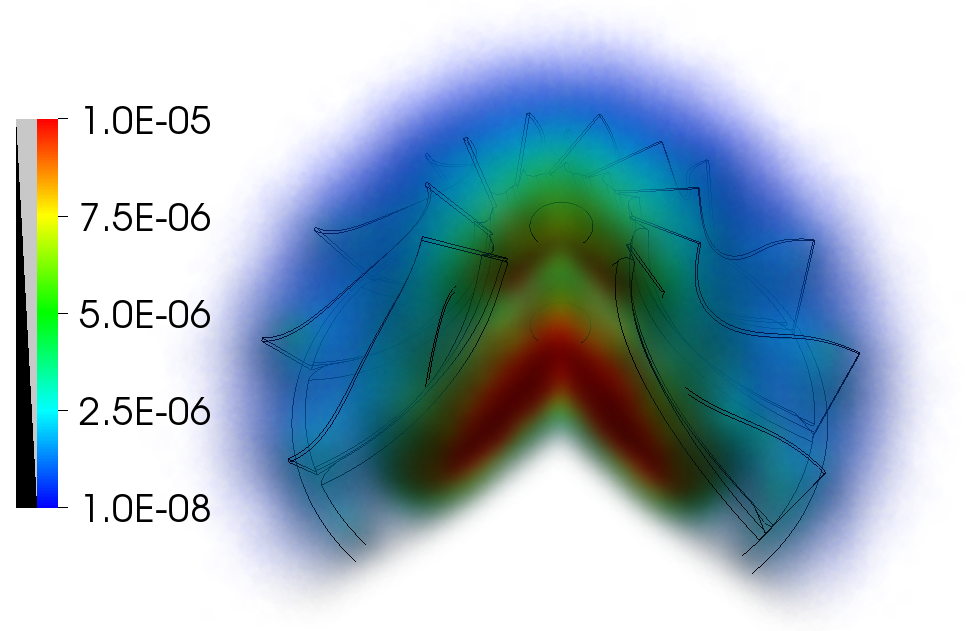
\includegraphics[height=7cm]{turbine_flux.png}}
\end{column}
\end{columns}

\end{frame}

%%%%%%%%%%%%%%%%%%%%%%%%%%%%%%%%%%%%%%%%%%%%%%%%%%%%%%
\begin{frame}{CADIS}
Consistant Adjoint-Driven Importance Sampling \cite{haghighat_monte_2003}
    \begin{itemize}
        \item{A Monte Carlo variance reduction technique that uses a deterministic estimate of the adjoint flux.}
        \begin{itemize}
            \item{Source biasing}
            \item{Weight windows}
        \end{itemize}
        \item{PyNE has a mesh-based implimentation:}
        \begin{itemize}
            \item{Uses the PyNE source sampling capabilities with MCNP for mesh-based source biasing.}
            \item{Adjoint fluxes from must be supplied, e.g. from the Denovo 3D S$_N$ code \cite{Evans2010}.}
        \end{itemize}    
    \end{itemize}
\end{frame}

%%%%%%%%%%%%%%%%%%%%%%%%%%%%%%%%%%%%%%%%%%%%%%%%%%%%%%
\begin{frame}
\frametitle{CADIS example}

\centering 
\hspace{0.7cm} source density \hspace{3.7cm} adjoint flux \\
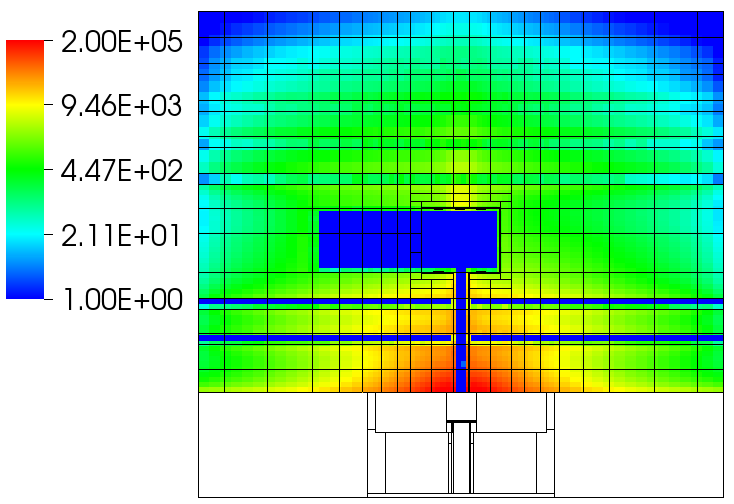
\includegraphics[width=4cm]{src.png} \hspace{1cm} 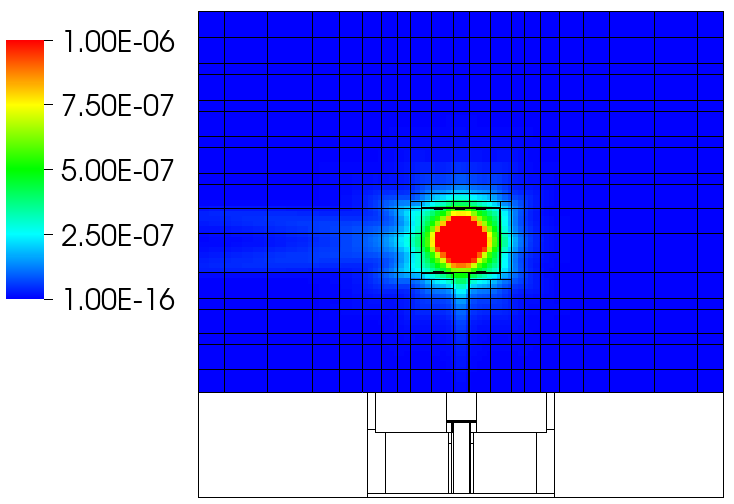
\includegraphics[width=4cm]{adj.png} \\
\vspace{0.3cm}
\hspace{0.5cm} \arrowdown CADIS \\
\vspace{0.3cm}
biased source density  \hspace{2cm} weight window lower bounds \\
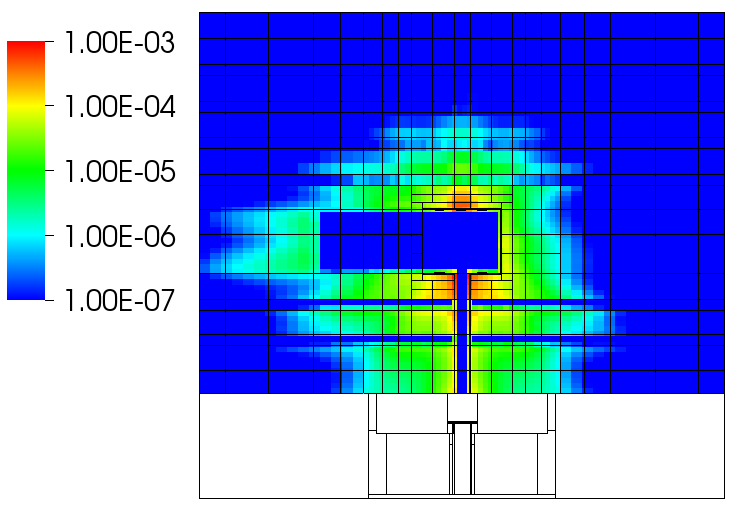
\includegraphics[width=4cm]{bsrc.png} \hspace{1cm}
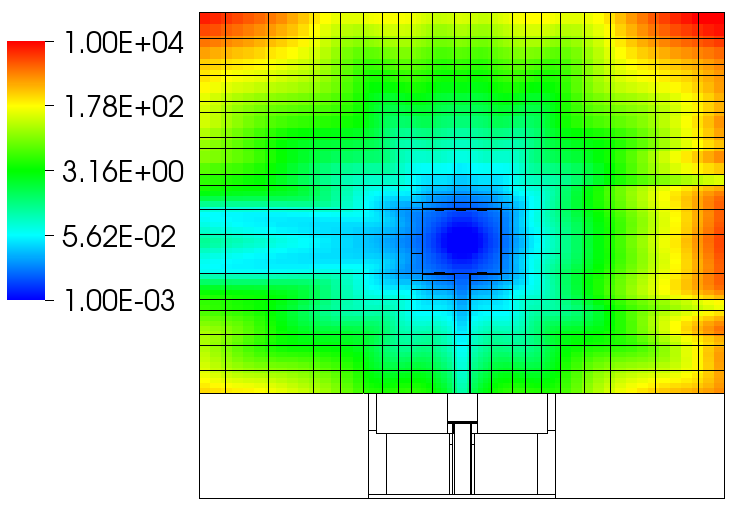
\includegraphics[width=4cm]{ww.png}

\end{frame}
%%%%%%%%%%%%%%%%%%%%%%%%%%%%%%%%%%%%%%%%%%%%%%%%%%%%%%
\begin{frame}{Rigorous Two-Step Activation}
    \begin{itemize}
        \item Neutrons activate system components, gamma source persists after shutdown.
        \item Important for occupational safety at ITER, JET, NIF, etc.
        \item DAG-MCNP5 \cite{wilson_acceleration_2009} for neutron and photon transport.
        \item ALARA \cite{wilson_alara_1999} for transmutation and decay.
    \end{itemize}

    \begin{columns}
        \begin{column}{0.5\textwidth}
            \centerline{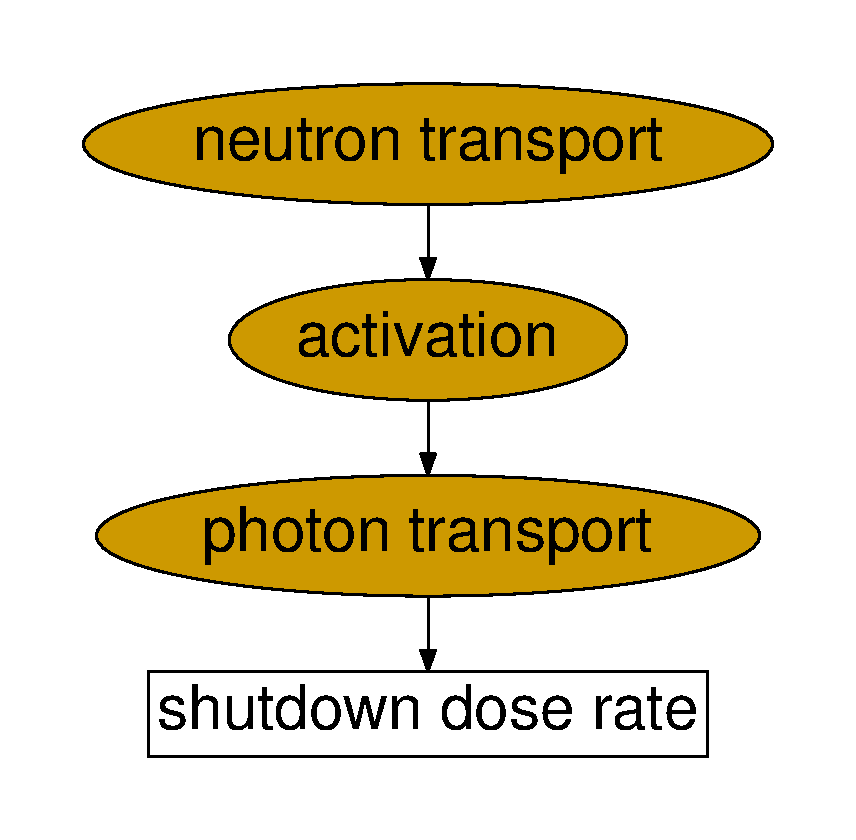
\includegraphics[height=0.5\textheight]{r2s.pdf}}
        \end{column}
        \begin{column}{0.5\textwidth}
            Uses the PyNE modules:
            \begin{itemize}
                \item{\texttt{mcnp}}
                \item{\texttt{mesh}}
                \item{\texttt{material} }
                \item{\texttt{alara}}
                \item{\texttt{dagmc}}
                \item{\texttt{source sampling}}
                \item{\texttt{variance reduction}}
                \item{\texttt{r2s module}}
           \end{itemize}
        \end{column}
    \end{columns}
\end{frame}
%%%%%%%%%%%%%%%%%%%%%%%%%%%%%%%%%%%%%%%%%%%%%%%%%%%%%%
\begin{frame}{Example: FNG ITER Shutdown Dose Rate Benchmark}
\centerline{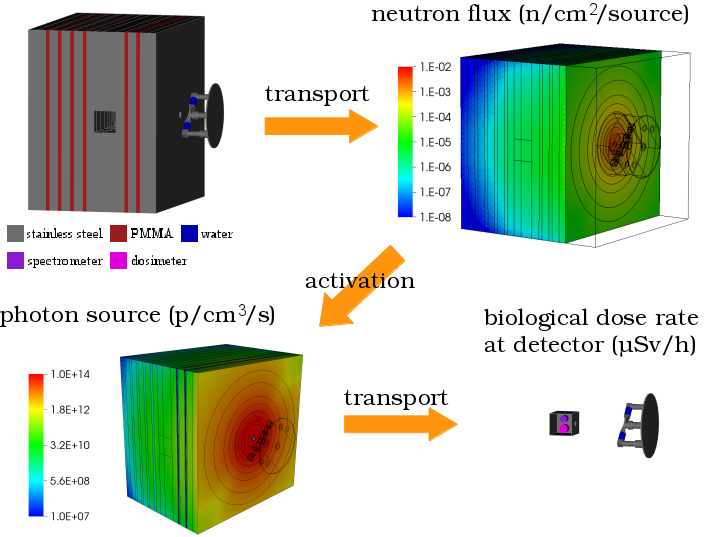
\includegraphics[height=0.85\textheight]{r2s_workflow.png}}
\end{frame}
%%%%%%%%%%%%%%%%%%%%%%%%%%%%%%%%%%%%%%%%%%%%%%%%%%%%%%
\begin{frame}{Comparison to Experimental Results}
    \begin{center}
        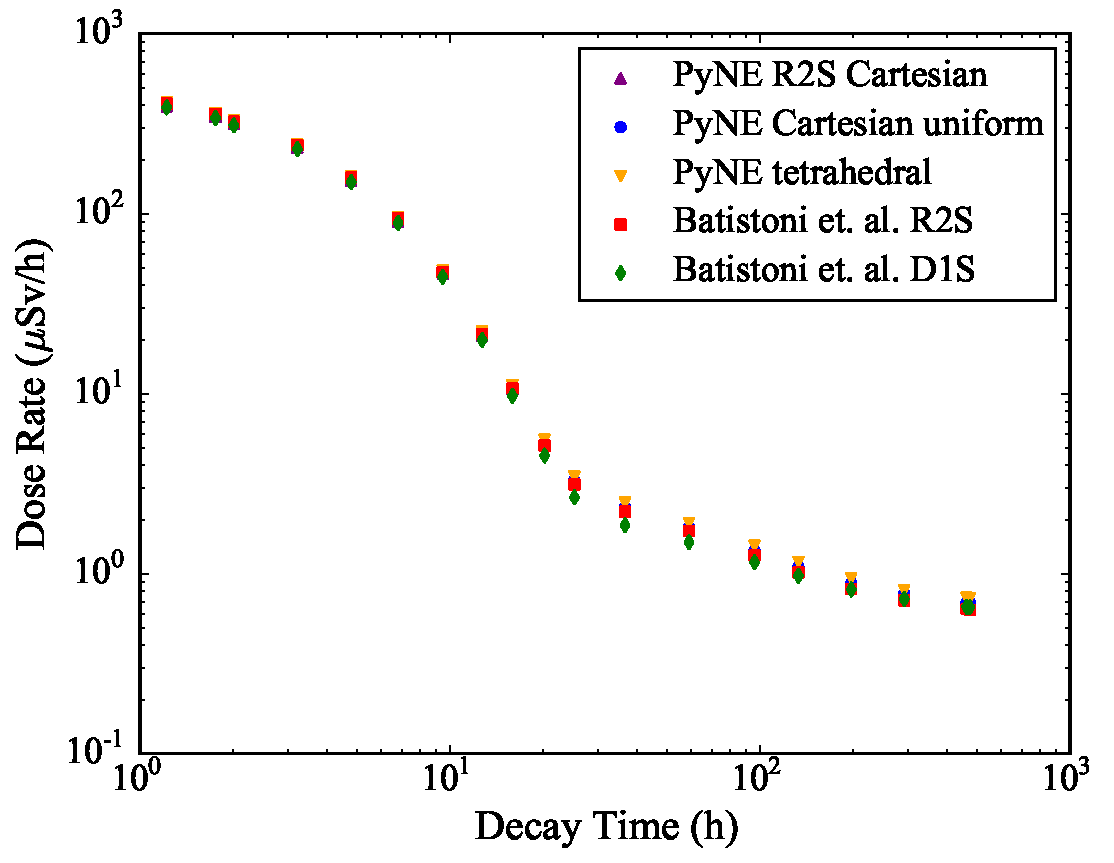
\includegraphics[height=2.5in,clip]{comp.pdf}
    \end{center}
\end{frame}
%%%%%%%%%%%%%%%%%%%%%%%%%%%%%%%%%%%%%%%%%%%%%%%%%%%%%%
%%%%%%%%%%%%%%%%%%%%%%%%%%%%%%%%%%%%%%%%%%%%%%%%%%%%%%

\begin{frame}{Installing PyNE}
  \Large
  \begin{itemize}
      \item Conda binary available (no compiler needed!)
      \item Ubuntu shell script
      \item Conda recipe (for developers)
      \item Single library (easier linking)
      \item Instructions for multiple platforms
      \item Relative links set during build
  \end{itemize}
\end{frame}


\begin{frame}{Even More Features!}
  \Large
    \begin{itemize}
        \item \texttt{fluka} support
        \item C++ amalgamation
        \item Tally container
        \item Python 3 support
        \item Continuous Integration (CI) testing
        \item Standardized style
        \item ACE 2.0.0 Header support
    \end{itemize}
\end{frame}


%\begin{frame}{Future Plans}
%    \begin{itemize}
%    \item Variance Reduction Workflows??
%    \item Plug and play transport tools/nuclear data
%    \item Wrap ENSDF utility/analysis codes
%    \item GND/FUDGE integration (Pending BSD license change)
%    \end{itemize}
%\end{frame}
%%%%%%%%%%%%%%%%%%%%%%%%%%%%%%%%%%%%%%%%%%%%%%%%%%%%%%
%%%%%%%%%%%%%%%%%%%%%%%%%%%%%%%%%%%%%%%%%%%%%%%%%%%%%%
%------------------------------------------------------


\section{Community Development}

\begin{frame}{Tutorials + Hackathons}
  \Large
    \begin{itemize}
        \item Tutorial - UC Berkeley Nov. 2013
        \begin{itemize}
            \large
            \item Engage Profs. and Grad + Educate Undergrads
        \end{itemize}
        \item 0.4 Sprint - UC Berkeley Feb. 2014
        \begin{itemize}
            \large
            \item Homogenizing code style
        \end{itemize}
        \item Tutorial - ANS RPSD 2014
        \begin{itemize}
            \large
            \item Engage national labs + industry
        \end{itemize}
        \item Hackathon - UC Berkeley Nov. 14-16
        \begin{itemize}
            \large
            \item Verification and Validation
        \end{itemize}
    \end{itemize}
\end{frame}

%%%%%%%%%%%%%%%%%%%%%%%%%%%%%%%%%%%%%%%%%%%%%%%%%%%%%%
%%%%%%%%%%%%%%%%%%%%%%%%%%%%%%%%%%%%%%%%%%%%%%%%%%%%%%

\section{Get involved!}
\begin{frame}{Why Would I Get Involved?}

\begin{block}{As a \alert{user}:}
    \begin{itemize}
    \item You could do your work or research with PyNE
    \item Even if you have your own software that looks and behaves similarly to some aspects of PyNE, using PyNE will mean that you no longer have to develop AND maintain that functionality
    \end{itemize}
\end{block}

    \vspace*{1 em}
\begin{block}{As a \alert{developer}:}
    \begin{itemize}
    \item You should be selfish
    \item Contribute to PyNE in ways that support the work that you are doing
    \item If a feature you want is not in PyNE right now, chances are that other
    people want to see that feature too
    \item This will help your future self as much as future other people
    \end{itemize}
\end{block}

\end{frame}

%------------------------------------------------------
\begin{frame}{How Can I Get Involved?}

    \begin{block}{\alert{Contact PyNE}}
    \begin{itemize}
    \item Website: \href{http://pyne.io/}{\texttt{http://pyne.io/}}

    \item User's Mailing List: \href{pyne-users@googlegroups.com}
    {\texttt{pyne-users@googlegroups.com}}

    \item Developer's List: \href{pyne-dev@googlegroups.com}
    {\texttt{pyne-dev@googlegroups.com}}

    \item GitHub: \href{https://github.com/pyne/pyne}
    {\texttt{https://github.com/pyne/pyne}}

    \item Tutorial: \href{http://pyne.io/tutorial/index.html}
    {\texttt{http://pyne.io/tutorial/index.html}}

%    \begin{itemize}
%    \item Website: \url{http://pyne.io/}
%    \item User's Mailing List: \href{mailto:pyne-users@googlegroups.com}{\nolinkurl{pyne-users@googlegroups.com}}
%    \item Developer's List: \href{mailto:pyne-dev@googlegroups.com}{\nolinkurl{pyne-dev@googlegroups.com}}
%    \item GitHub: \url{https://github.com/pyne/pyne}
    \end{itemize}
    \end{block}

    \vspace*{2 em}
    \begin{block}{\alert{What goes into PyNE?}}
    Anything that is not export controllable, proprietary,
    or under HIPPA restrictions!  (If you have questions, \emph{ask})
    \end{block}

\end{frame}

\begin{frame}[fragile]{Acknowledgements}
  \begin{itemize}
      \item PyNE is a diverse collection of knowledge
      \item We need lots of specialist to fill in the gaps:
  \end{itemize}

\small
  Anthony~Scopatz$^{1}$, Cameron~R.~Bates$^{2,3}$,
  Elliott~Biondo$^{1}$, Kathryn~Huff$^{2}$,
  Kalin Kiesling$^{1}$,
  Robert Carlsen$^{1}$,
  Andrew Davis$^{1}$,
  Matthew Gidden$^{1}$,
  Tim Haines$^{1}$,
  Joshua Howland$^{2}$,
  Blake Huff$^{2}$,
  Kevin Manalo$^{4}$,
  Arielle Opotowsky$^{1}$,
  Rachel Slaybaugh$^{2}$,
  Eric Relson$^{1}$,
  Paul Romano$^{5}$,
  Patrick Shriwise$^{1}$,
  John D. Xia$^{6}$,
  Paul Wilson$^{1}$,
  Julie Zachman$^{1}$\\
\vspace{0.2in}
\footnotesize
$^{1}$ The University of Wisconsin-Madison\\
$^{2}$ The University of California, Berkeley\\
$^{3}$ Lawrence Livermore National Laboratory\\
$^{4}$ Georgia Institute of Technology\\
$^{5}$ Massachusetts Institute of Technology\\
$^{6}$ University of Chicago

\end{frame}

%%%%%%%%%%%%%%%%%%%%%%%%%%%%%%%%%%%%%%%%%%%%%%%%%%%%%%
%%%%%%%%%%%%%%%%%%%%%%%%%%%%%%%%%%%%%%%%%%%%%%%%%%%%%%
\section*{}
\begin{frame}[fragile]{Questions?}

    \begin{center}
    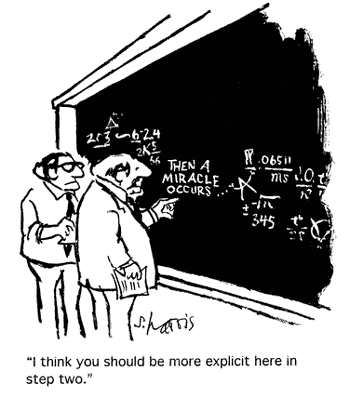
\includegraphics[height=3in,clip]{questions-comic.png}
    \end{center}

\end{frame}

% --------------------------------------------------------------
\begin{frame}[fragile]{PyNE In the Literature}

    \begin{itemize}
    \item Intro: ``PyNE: Python For Nuclear Engineering'' \cite{pyne_intro}
    \item Progress reports: \cite{scopatz_pyne}, \cite{pyne_progress}
    \item In research: \cite{Biondo2014}, \cite{MarquezDamian2014280}, \cite{Scopatz2013a}
    \item V\&V: ``Quality Assurance within the PyNE Open Source \\Toolkit'' \cite{pyne_vnv}
    \item Poster at SciPy: \cite{scipy}
    \end{itemize}

\end{frame}
% --------------------------------------------------------------
\begin{frame}[allowframebreaks]{References}
	\bibliographystyle{unsrt}
	\bibliography{answinter.bib}
\end{frame}

\end{document}
